% ============================================================================
% Diagrama Entidad-Relacion (notacion de Chen extendida con AGREGACIONES)
% Proyecto Final Bases de Datos - Inventario, Compras y Ventas (PostgreSQL)
% Compilar con: pdflatex diagrama_er.tex   (o pegar en Overleaf)
% ============================================================================
\documentclass[tikz,border=20pt]{standalone}
\usepackage[utf8]{inputenc}
\usepackage[T1]{fontenc}
\renewcommand{\familydefault}{\sfdefault}
\usetikzlibrary{shapes.geometric,shapes.multipart,calc,shadows,fit,backgrounds}

% ---------- capas (zonas < agregaciones < dibujo) ----------
\pgfdeclarelayer{zonas}
\pgfdeclarelayer{agr}
\pgfsetlayers{zonas,agr,main}

% ---------- paleta por microservicio / esquema ----------
\definecolor{cCat}{HTML}{2F6DB5}   % catalogo
\definecolor{cCom}{HTML}{E07B00}   % compras
\definecolor{cInv}{HTML}{2E8B57}   % inventarios
\definecolor{cVen}{HTML}{C0392B}   % ventas
\definecolor{cIde}{HTML}{7B4FB5}   % identidad
\definecolor{cRep}{HTML}{4A5560}   % reportes

% ---------- estilos ----------
\tikzset{
  ent/.style={draw=black!70, thick, rectangle split, rectangle split parts=2,
              font=\small, align=left, inner sep=5pt, text width=4.4cm,
              drop shadow={opacity=.18, shadow xshift=1.3pt, shadow yshift=-1.3pt}},
  entC/.style={ent, draw=cCat!75!black, rectangle split part fill={cCat!35, cCat!6}},
  entK/.style={ent, draw=cCom!75!black, rectangle split part fill={cCom!40, cCom!7}},
  entI/.style={ent, draw=cInv!75!black, rectangle split part fill={cInv!38, cInv!7}},
  entV/.style={ent, draw=cVen!75!black, rectangle split part fill={cVen!35, cVen!6}},
  entU/.style={ent, draw=cIde!75!black, rectangle split part fill={cIde!38, cIde!7}},
  rel/.style={draw=black!70, thick, diamond, aspect=2.4, font=\footnotesize, align=center,
              inner sep=0pt, minimum width=3.1cm, minimum height=1.35cm, fill=yellow!25},
  att/.style={draw=black!60, ellipse, fill=white, font=\scriptsize, inner sep=1.8pt,
              minimum height=.62cm},
  datt/.style={att, densely dashed},
  card/.style={font=\bfseries\footnotesize, fill=white, inner sep=1.3pt},
  fisica/.style={thick, black!85},
  logica/.style={thick, densely dashed, black!60},
  aline/.style={thin, black!55},
  zone/.style={rounded corners=10pt, draw=#1!65, fill=#1!5, thick,
               dash pattern=on 9pt off 4pt, inner sep=15pt},
  ztab/.style={font=\footnotesize\bfseries, text=white, fill=#1!80!black,
               rounded corners=3pt, inner sep=3.5pt, anchor=south west},
  agr/.style={draw=#1!80!black, very thick, dash pattern=on 5pt off 2.5pt,
              rounded corners=6pt, fill=#1!12, inner sep=6pt},
  agrtab/.style={font=\tiny\bfseries, text=#1!70!black, anchor=south west, inner sep=1.5pt}
}
\newcommand{\pk}[1]{\underline{#1}}
\newcommand{\fk}{\textsuperscript{\tiny FK}}
\newcommand{\uq}{\textsuperscript{\tiny U}}
% \entity{estilo}{id}{posicion}{esquema}{nombre}{atributos}
\newcommand{\entity}[6]{\node[#1] (#2) at (#3)
  {{\centering{\fontsize{6}{7}\selectfont\color{black!55}\ttfamily #4.}\\[-1pt]\textbf{#5}\par}%
   \nodepart{second}#6};}
% \zone{color}{id}{etiqueta}{lista fit}
\newcommand{\zone}[4]{\begin{pgfonlayer}{zonas}
  \node[zone=#1, fit=#4] (#2) {};
  \node[ztab=#1] at ([xshift=12pt]#2.north west) {#3};\end{pgfonlayer}}

\begin{document}
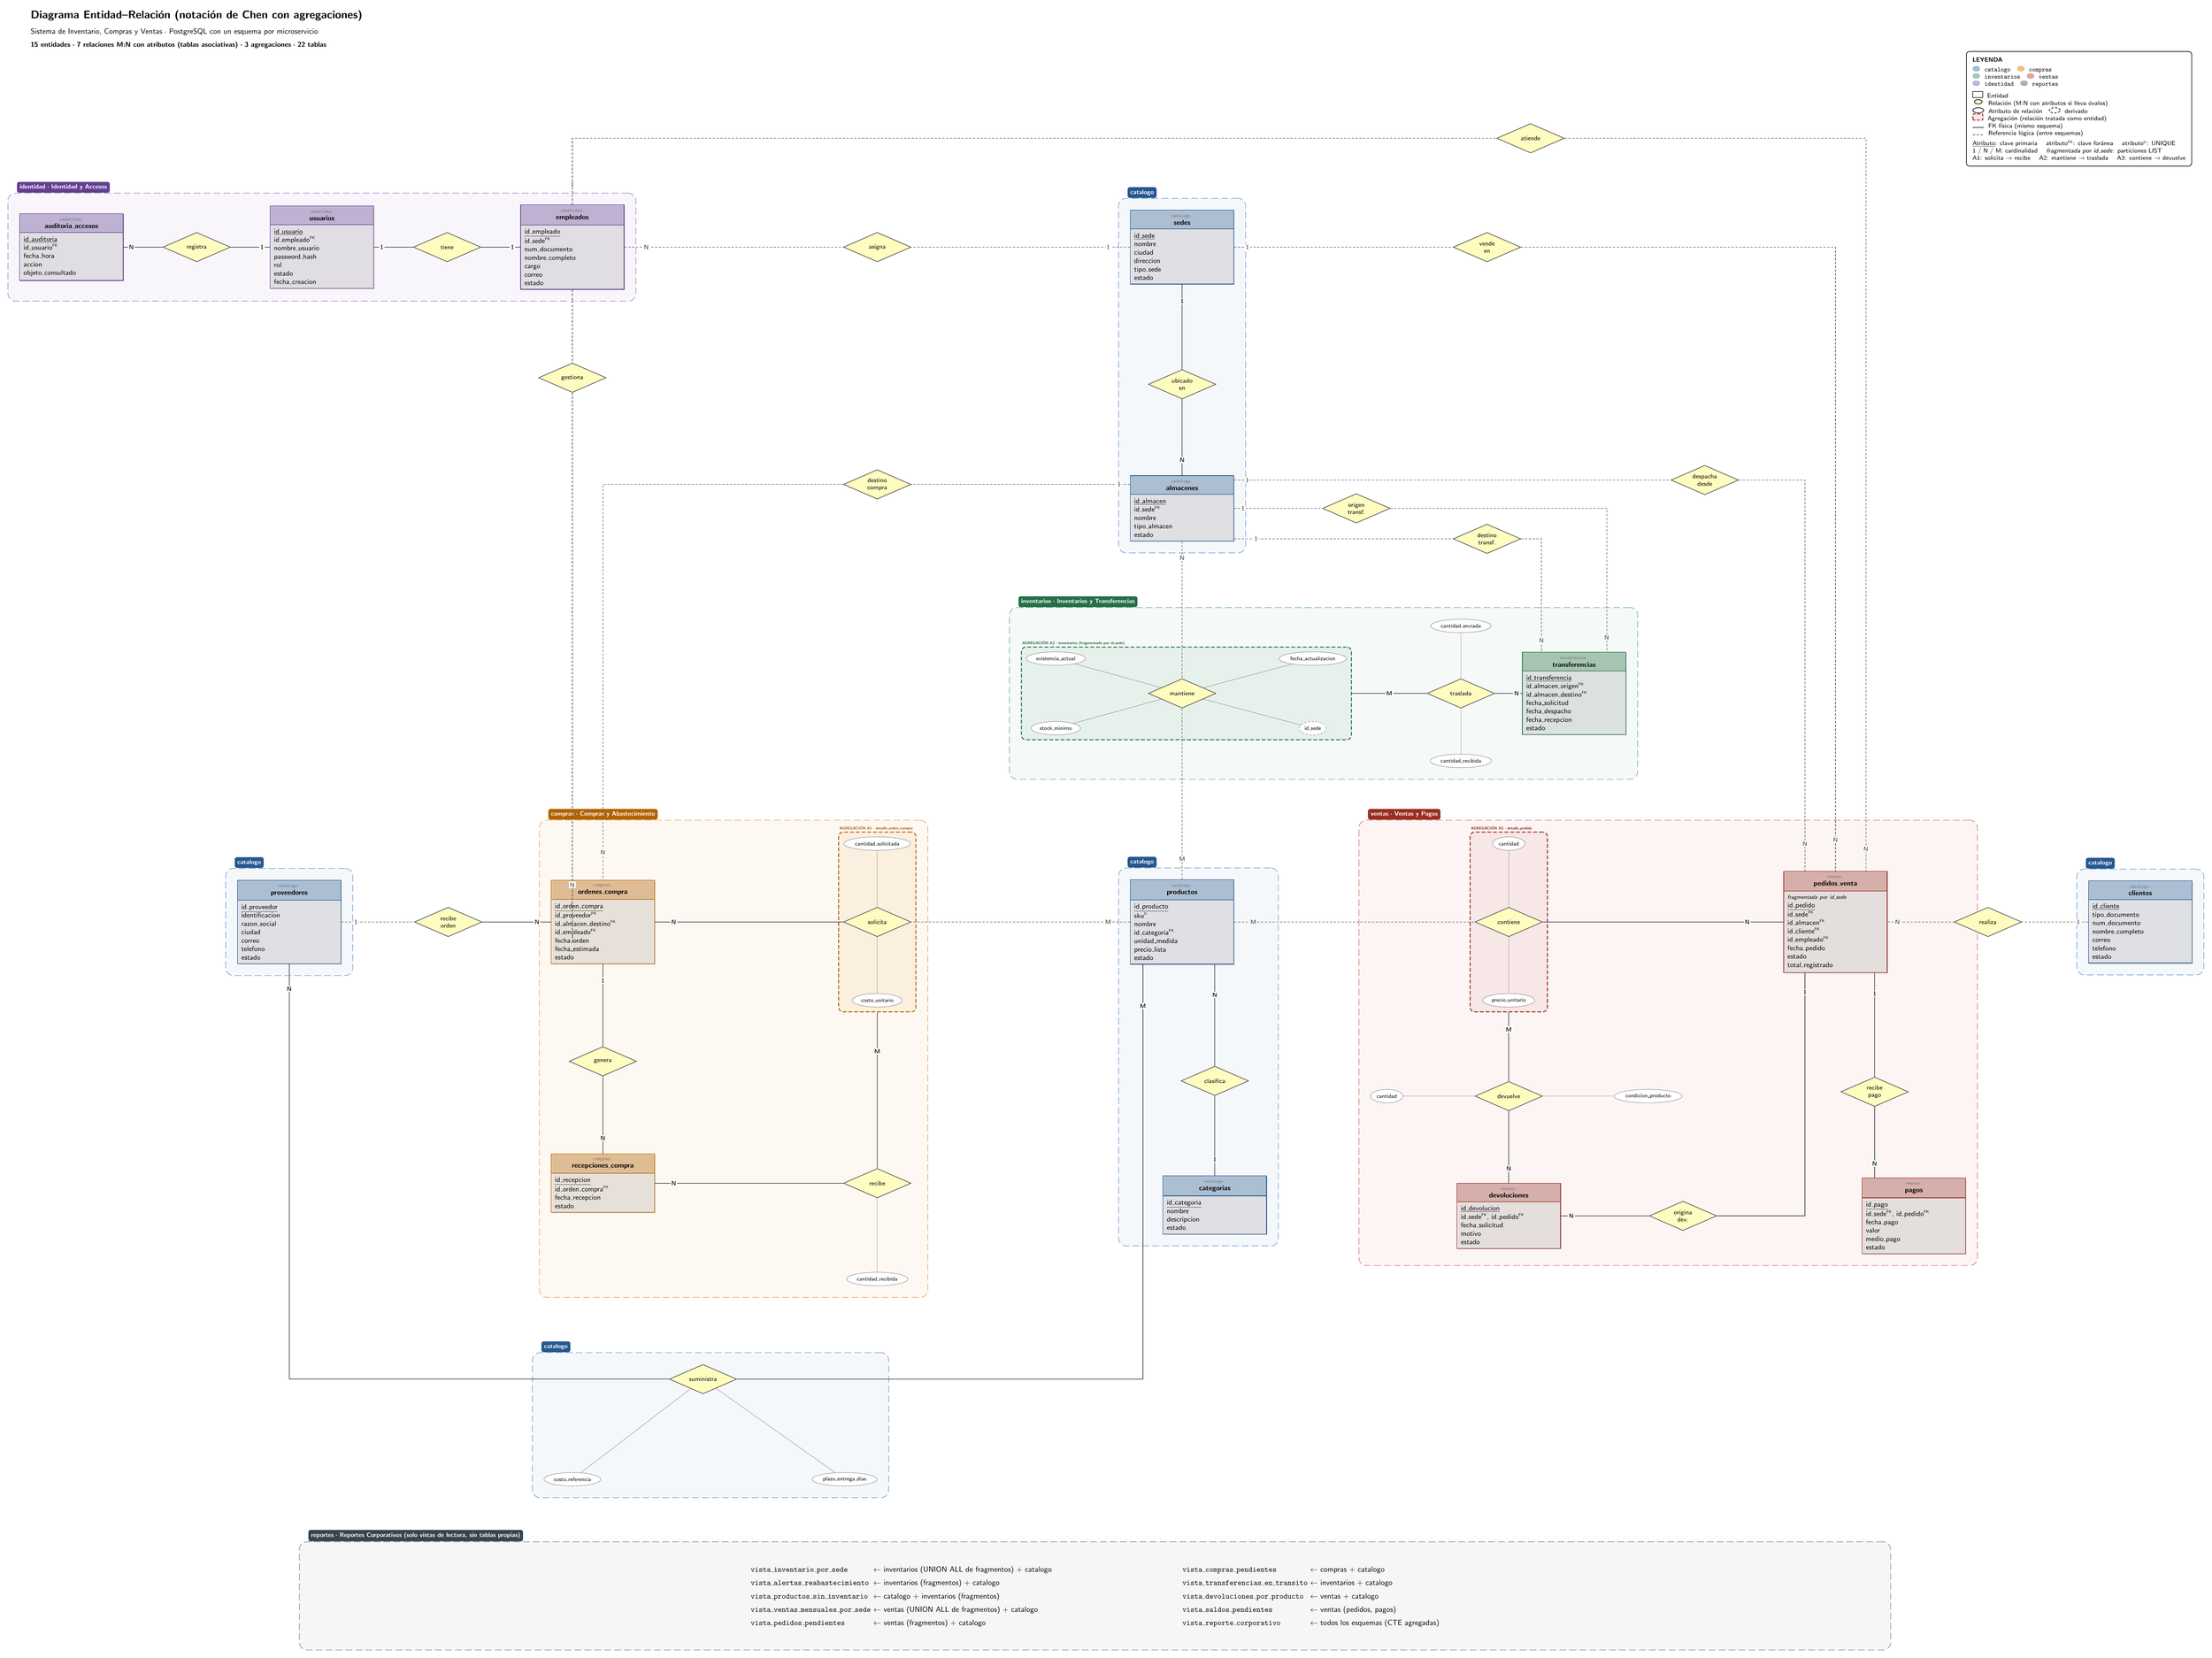
\begin{tikzpicture}

% =====================================================================
% ENTIDADES
% =====================================================================
% --- identidad ---
\entity{entU}{aud}{-7,0}{identidad}{auditoria\_accesos}
  {\pk{id\_auditoria}\\id\_usuario\fk\\fecha\_hora\\accion\\objeto\_consultado}
\entity{entU}{usu}{4.5,0}{identidad}{usuarios}
  {\pk{id\_usuario}\\id\_empleado\fk\\nombre\_usuario\\password\_hash\\rol\\estado\\fecha\_creacion}
\entity{entU}{emp}{16,0}{identidad}{empleados}
  {\pk{id\_empleado}\\id\_sede\fk\\num\_documento\\nombre\_completo\\cargo\\correo\\estado}
% --- catalogo ---
\entity{entC}{sed}{44,0}{catalogo}{sedes}
  {\pk{id\_sede}\\nombre\\ciudad\\direccion\\tipo\_sede\\estado}
\entity{entC}{alm}{44,-12}{catalogo}{almacenes}
  {\pk{id\_almacen}\\id\_sede\fk\\nombre\\tipo\_almacen\\estado}
\entity{entC}{pro}{44,-31}{catalogo}{productos}
  {\pk{id\_producto}\\sku\uq\\nombre\\id\_categoria\fk\\unidad\_medida\\precio\_lista\\estado}
\entity{entC}{cat}{45.5,-44}{catalogo}{categorias}
  {\pk{id\_categoria}\\nombre\\descripcion\\estado}
\entity{entC}{prv}{3,-31}{catalogo}{proveedores}
  {\pk{id\_proveedor}\\identificacion\\razon\_social\\ciudad\\correo\\telefono\\estado}
\entity{entC}{cli}{88,-31}{catalogo}{clientes}
  {\pk{id\_cliente}\\tipo\_documento\\num\_documento\\nombre\_completo\\correo\\telefono\\estado}
% --- compras ---
\entity{entK}{oc}{17.4,-31}{compras}{ordenes\_compra}
  {\pk{id\_orden\_compra}\\id\_proveedor\fk\\id\_almacen\_destino\fk\\id\_empleado\fk\\fecha\_orden\\fecha\_estimada\\estado}
\entity{entK}{rc}{17.4,-43}{compras}{recepciones\_compra}
  {\pk{id\_recepcion}\\id\_orden\_compra\fk\\fecha\_recepcion\\estado}
% --- inventarios ---
\entity{entI}{tr}{62,-20.5}{inventarios}{transferencias}
  {\pk{id\_transferencia}\\id\_almacen\_origen\fk\\id\_almacen\_destino\fk\\fecha\_solicitud\\fecha\_despacho\\fecha\_recepcion\\estado}
% --- ventas ---
\entity{entV}{pv}{74,-31}{ventas}{pedidos\_venta}
  {\textit{\scriptsize fragmentada por id\_sede}\\\pk{id\_pedido}\\id\_sede\fk\\id\_almacen\fk\\id\_cliente\fk\\id\_empleado\fk\\fecha\_pedido\\estado\\total\_registrado}
\entity{entV}{dev}{59,-44.5}{ventas}{devoluciones}
  {\pk{id\_devolucion}\\id\_sede\fk, id\_pedido\fk\\fecha\_solicitud\\motivo\\estado}
\entity{entV}{pag}{77.6,-44.5}{ventas}{pagos}
  {\pk{id\_pago}\\id\_sede\fk, id\_pedido\fk\\fecha\_pago\\valor\\medio\_pago\\estado}

% =====================================================================
% RELACIONES (rombos) Y AGREGACIONES
% =====================================================================
% --- identidad ---
\node[rel] (registra) at (-1.25,0) {registra};
\node[rel] (tiene)    at (10.25,0) {tiene};
\node[rel] (asigna)   at (30,0) {asigna};
\node[rel] (gestiona) at (16,-6) {gestiona};
% --- catalogo ---
\node[rel] (ubicado)  at (44,-6.3) {ubicado\\en};
\node[rel] (clasifica) at (45.5,-38.3) {clasifica};
\node[rel] (suministra) at (22,-52) {suministra};
\node[att] (s1) at (16,-56.6) {costo\_referencia};
\node[att] (s2) at (28.5,-56.6) {plazo\_entrega\_dias};
% --- compras ---
\node[rel] (recibeorden) at (10.3,-31) {recibe\\orden};
\node[rel] (destcompra)  at (30,-10.9) {destino\\compra};
\node[rel] (solicita) at (30,-31) {solicita};
\node[att] (a11) at (30,-27.4) {cantidad\_solicitada};
\node[att] (a12) at (30,-34.6) {costo\_unitario};
\node[rel] (genera)  at (17.4,-37.4) {genera};
\node[rel] (recibe)  at (30,-43) {recibe};
\node[att] (a13) at (30,-47.4) {cantidad\_recibida};
% --- inventarios ---
\node[rel] (mantiene) at (44,-20.5) {mantiene};
\node[att]  (b1) at (38.2,-18.9) {existencia\_actual};
\node[att]  (b2) at (38.2,-22.1) {stock\_minimo};
\node[att]  (b3) at (50,-18.9) {fecha\_actualizacion};
\node[datt] (b4) at (50,-22.1) {id\_sede};
\node[rel] (traslada) at (56.8,-20.5) {traslada};
\node[att] (c1) at (56.8,-17.4) {cantidad\_enviada};
\node[att] (c2) at (56.8,-23.6) {cantidad\_recibida};
\node[rel] (origen)  at (52,-12) {origen\\transf.};
\node[rel] (destino) at (58,-13.4) {destino\\transf.};
% --- ventas ---
\node[rel] (realiza)  at (81,-31) {realiza};
\node[rel] (despacha) at (68,-10.7) {despacha\\desde};
\node[rel] (vendeen)  at (58,0) {vende\\en};
\node[rel] (atiende)  at (60,5) {atiende};
\node[rel] (contiene) at (59,-31) {contiene};
\node[att] (d1) at (59,-27.4) {cantidad};
\node[att] (d2) at (59,-34.6) {precio\_unitario};
\node[rel] (devuelve) at (59,-39) {devuelve};
\node[att] (e1) at (53.4,-39) {cantidad};
\node[att] (e2) at (65.4,-39) {condicion\_producto};
\node[rel] (origina) at (67,-44.5) {origina\\dev.};
\node[rel] (recpago) at (75.8,-38.8) {recibe\\pago};

% --- cajas de agregacion ---
\begin{pgfonlayer}{agr}
  \node[agr=cCom, fit=(solicita)(a11)(a12)] (A1) {};
  \node[agrtab=cCom] at (A1.north west) {AGREGACIÓN A1 · detalle\_orden\_compra};
  \node[agr=cInv, fit=(mantiene)(b1)(b2)(b3)(b4)] (A2) {};
  \node[agrtab=cInv] at (A2.north west) {AGREGACIÓN A2 · inventarios (fragmentada por id\_sede)};
  \node[agr=cVen, fit=(contiene)(d1)(d2)] (A3) {};
  \node[agrtab=cVen] at (A3.north west) {AGREGACIÓN A3 · detalle\_pedido};
\end{pgfonlayer}

% =====================================================================
% LINEAS  (continua = FK fisica en el esquema; punteada = referencia logica)
% =====================================================================
% atributos de relaciones
\foreach \a/\r in {s1/suministra,s2/suministra,a11/solicita,a12/solicita,a13/recibe,
  b1/mantiene,b2/mantiene,b3/mantiene,b4/mantiene,c1/traslada,c2/traslada,
  d1/contiene,d2/contiene,e1/devuelve,e2/devuelve}
  \draw[aline] (\a) -- (\r);

% --- identidad ---
\draw[fisica] (usu.west) -- node[card,pos=.2]{1} (registra);
\draw[fisica] (aud.east) -- node[card,pos=.2]{N} (registra);
\draw[fisica] (emp.west) -- node[card,pos=.2]{1} (tiene);
\draw[fisica] (usu.east) -- node[card,pos=.2]{1} (tiene);
\draw[logica] (sed.west) -- node[card,pos=.1]{1} (asigna);
\draw[logica] (emp.east) -- node[card,pos=.1]{N} (asigna);
% --- catalogo ---
\draw[fisica] (sed.south) -- node[card,pos=.2]{1} (ubicado);
\draw[fisica] (alm.north) -- node[card,pos=.2]{N} (ubicado);
\draw[fisica] (cat.north) -- node[card,pos=.2]{1} (clasifica);
\draw[fisica] ($(pro.south)+(1.5,0)$) -- node[card,pos=.3]{N} (clasifica);
\draw[fisica] (prv.south) -- node[card,pos=.06]{N} (3,-52) -- (suministra);
\draw[fisica] (suministra) -- (42.2,-52) -- node[card,pos=.9]{M} ($(pro.south)+(-1.8,0)$);
% --- compras ---
\draw[logica] (prv.east) -- node[card,pos=.2]{1} (recibeorden);
\draw[fisica] (oc.west) -- node[card,pos=.2]{N} (recibeorden);
\draw[logica] (emp.south) -- node[card,pos=.15]{1} (gestiona);
\draw[logica] (gestiona) -- ($(emp.south)+(0,-30)$) -- node[card,pos=.92]{N} ($(oc.north)+(-1.4,0)$);
\draw[logica] ($(alm.west)+(0,1.1)$) -- node[card,pos=.05]{1} (destcompra);
\draw[logica] (destcompra) -- (17.4,-10.9) -- node[card,pos=.93]{N} (oc.north);
\draw[fisica] (oc.east) -- node[card,pos=.1]{N} (solicita);
\draw[logica] (pro.west) -- node[card,pos=.1]{M} (solicita);
\draw[fisica] (oc.south) -- node[card,pos=.2]{1} (genera);
\draw[fisica] (rc.north) -- node[card,pos=.2]{N} (genera);
\draw[fisica] (rc.east) -- node[card,pos=.1]{N} (recibe);
\draw[fisica] (recibe) -- node[card,pos=.75]{M} (A1.south);
% --- inventarios ---
\draw[logica] (alm.south) -- node[card,pos=.12]{N} (mantiene);
\draw[logica] (pro.north) -- node[card,pos=.12]{M} (mantiene);
\draw[fisica] (A2.east) -- node[card,pos=.5]{M} (traslada);
\draw[fisica] (tr.west) -- node[card,pos=.2]{N} (traslada);
\draw[logica] (alm.east) -- node[card,pos=.1]{1} (origen);
\draw[logica] (origen) -- (63.5,-12) -- node[card,pos=.9]{N} ($(tr.north)+(1.5,0)$);
\draw[logica] ($(alm.east)+(0,-1.4)$) -- node[card,pos=.1]{1} (destino);
\draw[logica] (destino) -- (60.5,-13.4) -- node[card,pos=.9]{N} ($(tr.north)+(-1.5,0)$);
% --- ventas ---
\draw[logica] (cli.west) -- node[card,pos=.15]{1} (realiza);
\draw[logica] (pv.east) -- node[card,pos=.15]{N} (realiza);
\draw[logica] ($(alm.east)+(0,1.3)$) -- node[card,pos=.03]{1} (despacha) -- (72.6,-10.7)
   -- node[card,pos=.93]{N} ($(pv.north)+(-1.4,0)$);
\draw[logica] (sed.east) -- node[card,pos=.06]{1} (vendeen) -- (74,0)
   -- node[card,pos=.95]{N} (pv.north);
\draw[logica] (emp.north) -- node[card,pos=.3]{1} (16,5) -- (atiende) -- (75.4,5)
   -- node[card,pos=.97]{N} ($(pv.north)+(1.4,0)$);
\draw[fisica] (pv.west) -- node[card,pos=.15]{N} (contiene);
\draw[logica] (pro.east) -- node[card,pos=.08]{M} (contiene);
\draw[fisica] ($(pv.south)+(-1.4,0)$) -- node[card,pos=.08]{1} (72.6,-44.5) -- (origina);
\draw[fisica] (dev.east) -- node[card,pos=.12]{N} (origina);
\draw[fisica] (dev.north) -- node[card,pos=.2]{N} (devuelve);
\draw[fisica] (devuelve) -- node[card,pos=.75]{M} (A3.south);
\draw[fisica] ($(pv.south)+(1.8,0)$) -- node[card,pos=.2]{1} (recpago);
\draw[fisica] ($(pag.north)+(-1.8,0)$) -- node[card,pos=.2]{N} (recpago);

% =====================================================================
% ZONAS (microservicios)
% =====================================================================
\zone{cIde}{zI}{identidad · Identidad y Accesos}{(aud)(usu)(emp)(registra)(tiene)}
\zone{cCom}{zK}{compras · Compras y Abastecimiento}{(oc)(rc)(A1)(recibe)(genera)(a13)}
\zone{cInv}{zN}{inventarios · Inventarios y Transferencias}{(A2)(tr)(traslada)(c1)(c2)}
\zone{cVen}{zV}{ventas · Ventas y Pagos}{(pv)(A3)(dev)(pag)(devuelve)(e1)(e2)}
\zone{cCat}{zC1}{catalogo}{(sed)(alm)(ubicado)}
\zone{cCat}{zC2}{catalogo}{(pro)(cat)(clasifica)}
\zone{cCat}{zC3}{catalogo}{(prv)}
\zone{cCat}{zC4}{catalogo}{(cli)}
\zone{cCat}{zC5}{catalogo}{(suministra)(s1)(s2)}

% =====================================================================
% REPORTES
% =====================================================================
\node[font=\normalsize, align=left, inner sep=12pt, anchor=north, minimum width=72cm] (rep) at (40,-60)
 {\renewcommand{\arraystretch}{1.45}%
  \begin{tabular}{@{}l@{\ $\leftarrow$\ }l@{\hspace{6cm}}l@{\ $\leftarrow$\ }l@{}}
  \texttt{vista\_inventario\_por\_sede} & inventarios (UNION ALL de fragmentos) + catalogo &
  \texttt{vista\_compras\_pendientes} & compras + catalogo\\
  \texttt{vista\_alertas\_reabastecimiento} & inventarios (fragmentos) + catalogo &
  \texttt{vista\_transferencias\_en\_transito} & inventarios + catalogo\\
  \texttt{vista\_productos\_sin\_inventario} & catalogo + inventarios (fragmentos) &
  \texttt{vista\_devoluciones\_por\_producto} & ventas + catalogo\\
  \texttt{vista\_ventas\_mensuales\_por\_sede} & ventas (UNION ALL de fragmentos) + catalogo &
  \texttt{vista\_saldos\_pendientes} & ventas (pedidos, pagos)\\
  \texttt{vista\_pedidos\_pendientes} & ventas (fragmentos) + catalogo &
  \texttt{vista\_reporte\_corporativo} & todos los esquemas (CTE agregadas)
  \end{tabular}};
\zone{cRep}{zR}{reportes · Reportes Corporativos (solo vistas de lectura, sin tablas propias)}{(rep)}

% =====================================================================
% TITULO Y LEYENDA
% =====================================================================
\node[font=\Large\bfseries, anchor=south west, align=left] at (-9,9)
  {Diagrama Entidad--Relación (notación de Chen con agregaciones)\\[2pt]
   \normalsize\mdseries Sistema de Inventario, Compras y Ventas · PostgreSQL con un esquema por microservicio\\[-1pt]
   \small 15 entidades · 7 relaciones M:N con atributos (tablas asociativas) · 3 agregaciones · 22 tablas};

\node[draw, thick, fill=white, align=left, font=\footnotesize, inner sep=8pt,
      rounded corners=4pt, anchor=north west] at (80,9) {\textbf{LEYENDA}\\[3pt]
  \tikz\fill[cCat!45] (0,0) rectangle (.35,.25); \ \texttt{catalogo}\quad
  \tikz\fill[cCom!50] (0,0) rectangle (.35,.25); \ \texttt{compras}\\
  \tikz\fill[cInv!45] (0,0) rectangle (.35,.25); \ \texttt{inventarios}\quad
  \tikz\fill[cVen!45] (0,0) rectangle (.35,.25); \ \texttt{ventas}\\
  \tikz\fill[cIde!45] (0,0) rectangle (.35,.25); \ \texttt{identidad}\quad
  \tikz\fill[cRep!45] (0,0) rectangle (.35,.25); \ \texttt{reportes}\\[4pt]
  \tikz\draw[thick,sharp corners] (0,0) rectangle (.45,.28); \ Entidad\\
  \tikz\draw[thick,fill=yellow!25] (.25,0) -- (.5,.14) -- (.25,.28) -- (0,.14) -- cycle; \ Relación (M:N con atributos si lleva óvalos)\\
  \tikz\draw[thick,fill=white] (.25,.14) ellipse (.25 and .12); \ Atributo de relación\quad
  \tikz\draw[thick,densely dashed,fill=white] (.25,.14) ellipse (.25 and .12); \ derivado\\
  \tikz\draw[very thick,cVen!80!black,dash pattern=on 4pt off 2pt,rounded corners=1pt,fill=cVen!12] (0,0) rectangle (.45,.28); \ Agregación (relación tratada como entidad)\\
  \tikz\draw[thick] (0,.1) -- (.5,.1); \ FK física (mismo esquema)\\
  \tikz\draw[thick,densely dashed,black!60] (0,.1) -- (.5,.1); \ Referencia lógica (entre esquemas)\\[4pt]
  \pk{Atributo}: clave primaria \quad atributo\fk: clave foránea \quad atributo\uq: UNIQUE\\
  1 / N / M: cardinalidad \quad \textit{fragmentada por id\_sede}: particiones LIST\\
  A1: solicita $\to$ recibe \quad A2: mantiene $\to$ traslada \quad A3: contiene $\to$ devuelve};

\end{tikzpicture}
\end{document}
